\newpage
\section{Growth}

Growth models are fundamental in understanding population dynamics, resource consumption, and many natural and artificial processes. Two primary models of growth are the \textbf{exponential} and the \textbf{logistic} growth models. Each of these has discrete and continuous forms.

\subsection{Exponential Growth}

Exponential growth describes a process that increases at a rate proportional to its current value.

\subsubsection{Discrete Exponential Growth}

\[
  P_{n} = P_0 \cdot (1 + r)^n
\]

Where:

\begin{itemize}

  \item \(P_n\) is the population at time step \emph{n}

  \item \(P_0\) is the initial population

  \item \(r\) is the growth rate per time step

  \item \emph{n} is the number of time steps

\end{itemize}

\textbf{Example:}
\vspace{\baselineskip}
  
If \(P_0 = 100\) and \(r = 0.1\), after 5 steps:

\[
  P_5 = 100 \cdot {(1 + 0.1)}^5 = 100 \cdot 1.61051 \approx 161.05
\]

\subsubsection{Continuous Exponential Growth}

  \[
P(t) = P_0 \cdot e^{rt}
\]

Where:

\begin{itemize}

  \item \(P(t)\) is the population at time \emph{t}

  \item \emph{e} is Euler’s number (\(\approx 2.718\))

  \item \(r\) is the continuous growth rate

\end{itemize}

\textbf{Example:}
\vspace{\baselineskip}
  
If \(P_0 = 100\), \(r = 0.1\), and \(t = 5\):

\[
    P(5) = 100 \cdot e^{0.5} \approx 100 \cdot 1.64872 \approx 164.87
\]

\begin{center}
    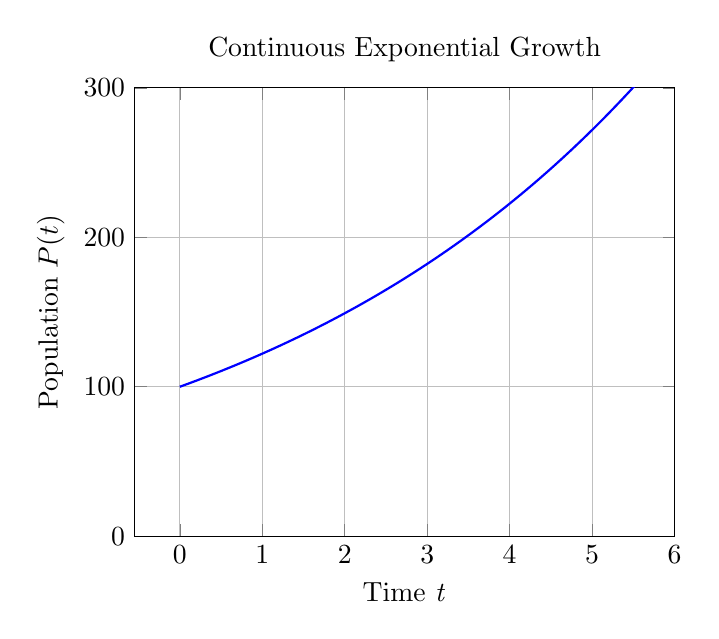
\begin{tikzpicture}
    \begin{axis}[
        xlabel={Time \emph{t}},
        ylabel={Population \(P(t)\)},
        title={Continuous Exponential Growth},
        domain=0:10,
        samples=100,
        ymin=0, ymax=300,
        grid=major,
    ]
    \addplot[blue, thick] {100*exp(0.2*x)};
    \end{axis}
    \end{tikzpicture}
\end{center}

\subsection{Logistic Growth}

Logistic growth occurs when a population grows rapidly at first and then slows as it approaches a maximum sustainable size (carrying capacity).

\subsubsection{Discrete Logistic Growth}

\[
    P_{n+1} = P_n + r \cdot P_n \cdot \left(1 - \frac{P_n}{K}\right)
\]

Where:

\begin{itemize}

  \item \(K\) is the carrying capacity

  \item \(r\) is the intrinsic growth rate

\end{itemize}

\textbf{Example:}
\vspace{\baselineskip}
  
With \(P_0 = 10\), \(r = 0.5\), \(K = 100\):

\[
    P_1 = 10 + 0.5 \cdot 10 \cdot \left(1 - \frac{10}{100}\right) = 10 + 0.5 \cdot 10 \cdot 0.9 = 10 + 4.5 = 14.5
\]

\begin{center}
    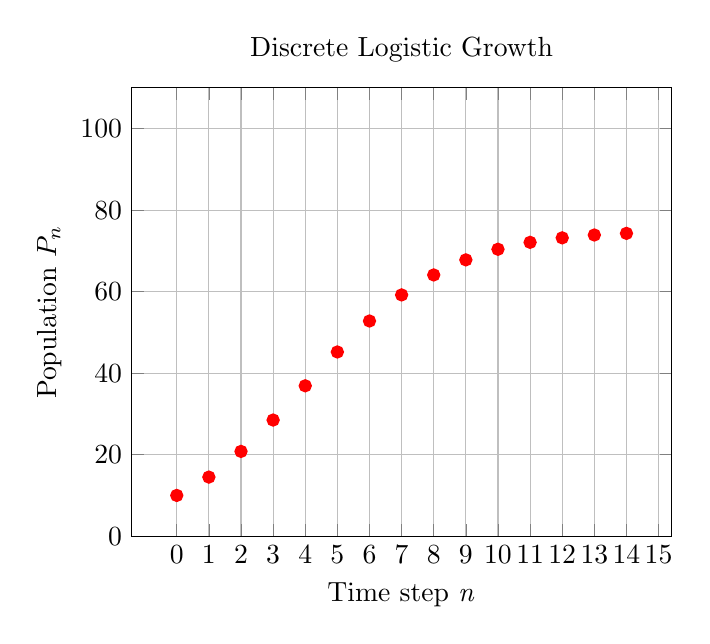
\begin{tikzpicture}
    \begin{axis}[
        xlabel={Time step \emph{n}},
        ylabel={Population \(P_n\)},
        title={Discrete Logistic Growth},
        ytick={0,20,...,100},
        ymin=0, ymax=110,
        xtick={0,1,...,20},
        grid=major,
    ]
    \addplot+[only marks, mark=*, mark options={red}, thick] 
        table [row sep=\\] {
        x  y \\
        0  10 \\
        1  14.5 \\
        2  20.8 \\
        3  28.5 \\
        4  36.9 \\
        5  45.2 \\
        6  52.8 \\
        7  59.2 \\
        8  64.1 \\
        9  67.8 \\
        10 70.4 \\
        11 72.1 \\
        12 73.2 \\
        13 73.9 \\
        14 74.3 \\
        };
    \end{axis}
    \end{tikzpicture}
\end{center}

\subsubsection{Continuous Logistic Growth}

\[
    P(t) = \frac{K}{1 + \left( \frac{K - P_0}{P_0} \right)e^{-rt}}
\]

\textbf{Example:}
\vspace{\baselineskip}
  
With \(P_0 = 10\), \(K = 100\), and \(r = 0.5\), at \(t = 5\):

\[
    P(5) = \frac{100}{1 + \left( \frac{90}{10} \right)e^{-0.5 \cdot 5}} = \frac{100}{1 + 9e^{-2.5}} \approx \frac{100}{1.7387} \approx 57.52
\]

\begin{center}
    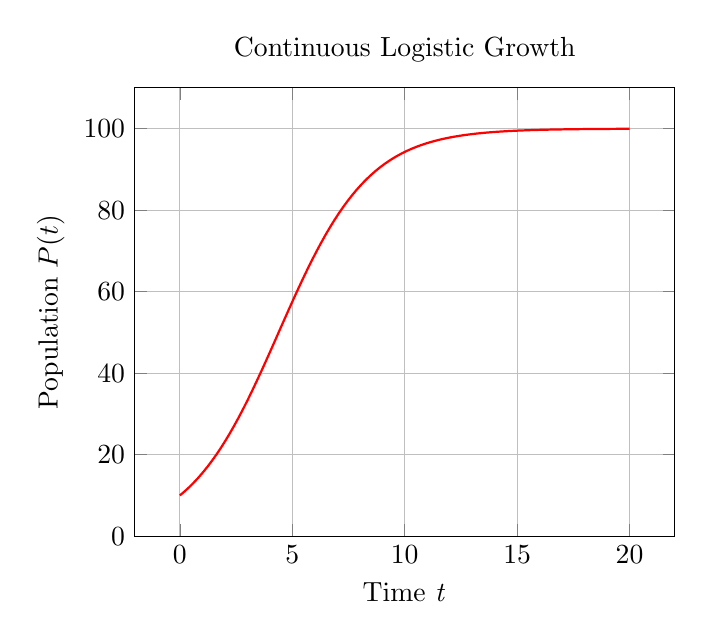
\begin{tikzpicture}
    \begin{axis}[
        xlabel={Time \emph{t}},
        ylabel={Population \(P(t)\)},
        title={Continuous Logistic Growth},
        domain=0:20,
        samples=100,
        ymin=0, ymax=110,
        grid=major,
    ]
    \addplot[red, thick] {100/(1 + (90/10)*exp(-0.5*x))};
    \end{axis}
    \end{tikzpicture}
\end{center}
